%  LaTeX support: latex@mdpi.com 
%  In case you need support, please attach all files that are necessary for compiling as well as the log file, and specify the details of your LaTeX setup (which operating system and LaTeX version / tools you are using).

% You need to save the "mdpi.cls" and "mdpi.bst" files into the same folder as this template file.

%=================================================================
\documentclass[bioengineering,article,submit,moreauthors,pdftex,10pt,a4paper]{mdpi} 
%
%--------------------
% Class Options:
%--------------------
% journal
%----------
% Choose between the following MDPI journals:
% actuators, admsci, aerospace, agriculture, agronomy, algorithms, animals, antibiotics, antibodies, antioxidants, applsci, arts, atmosphere, atoms, axioms, batteries, bdcc, behavsci, beverages, bioengineering, biology, biomedicines, biomimetics, biomolecules, biosensors, brainsci, buildings, carbon, cancers, catalysts, cells, challenges, chemengineering, chemosensors, children, chromatography, climate, coatings, computation, computers, condensedmatter, cosmetics, cryptography, crystals, data, dentistry, designs, diagnostics, diseases, diversity, econometrics, economies, education, electronics, energies, entropy, environments, epigenomes, fermentation, fibers, fishes, fluids, foods, forests, fractalfract, futureinternet, galaxies, games, gastrointestdisord, gels, genealogy, genes, geosciences, geriatrics, healthcare, horticulturae, humanities, hydrology, informatics, information, infrastructures, inorganics, insects, instruments, ijerph, ijfs, ijms, ijgi, ijtpp, inventions, jcdd, jcm, jcs, jdb, jfb, jfmk, jimaging, jof, jintelligence, jlpea, jmse, jpm, jrfm, jsan, land, languages, laws, life, literature, logistics, lubricants, machines, magnetochemistry, marinedrugs, materials, mathematics, mca, mti, medsci, medicines, membranes, metabolites, metals, microarrays, micromachines, microorganisms, minerals, molbank, molecules, mps, nanomaterials, ncrna, neonatalscreening, nitrogen, nutrients, ohbm, particles, pathogens, pharmaceuticals, pharmaceutics, pharmacy, philosophies, photonics, plants, polymers, proceedings, processes, proteomes, publications, quaternary, qubs, recycling, religions, remotesensing, resources, risks, robotics, safety, scipharm, sensors, separations, sexes, sinusitis, socsci, societies, soils, sports, standards, sustainability, symmetry, systems, technologies, toxics, toxins, tropicalmed, universe, urbansci, vaccines, vetsci, viruses, vision, water
%---------
% article
%---------
% The default type of manuscript is article, but can be replaced by: 
% addendum, article, book, bookreview, briefreport, casereport, changes, comment, commentary, communication, conceptpaper, correction, conferenceproceedings, conferencereport, expressionofconcern, meetingreport, creative, datadescriptor, discussion, editorial, essay, erratum, hypothesis, interestingimage, letter, newbookreceived, opinion, obituary, projectreport, reply, reprint, retraction, review, perspective, preprints, shortnote, supfile, technicalnote, viewpoint
% supfile = supplementary materials
%----------
% submit
%----------
% The class option "submit" will be changed to "accept" by the Editorial Office when the paper is accepted. This will only make changes to the frontpage (e.g. the logo of the journal will get visible), the headings, and the copyright information. Also, line numbering will be removed. Journal info and pagination for accepted papers will also be assigned by the Editorial Office.
%------------------
% moreauthors
%------------------
% If there is only one author the class option oneauthor should be used. Otherwise use the class option moreauthors.
%---------
% pdftex
%---------
% The option pdftex is for use with pdfLaTeX. If eps figure are used, remove the option pdftex and use LaTeX and dvi2pdf.

%=================================================================
\firstpage{1} 
\makeatletter 
\setcounter{page}{\@firstpage} 
\makeatother 
\articlenumber{x}
\doinum{10.3390/------}
\pubvolume{xx}
\pubyear{2017}
\copyrightyear{2017}
%\externaleditor{Academic Editor: name}
\history{Received: date; Accepted: date; Published: date}

%------------------------------------------------------------------
% The following line should be uncommented if the LaTeX file is uploaded to arXiv.org
%\pdfoutput=1

%=================================================================
% Add packages and commands here. The following packages are loaded in our class file: fontenc, calc, indentfirst, fancyhdr, graphicx, lastpage, ifthen, lineno, float, amsmath, setspace, enumitem, mathpazo, booktabs, titlesec, etoolbox, amsthm, hyphenat, natbib, hyperref, footmisc, geometry, caption, url, mdframed, tabto, soul, multirow, microtype

%=================================================================
%% Please use the following mathematics environments: Theorem, Lemma, Corollary, Proposition, Characterization, Property, Problem, Example, ExamplesandDefinitions, Hypothesis, Remark, Definition
%% For proofs, please use the proof environment (the amsthm package is loaded by the MDPI class).

%=================================================================
% Full title of the paper (Capitalized)
\Title{A Fuzzy Approach for Term and Preterm Identification}

% If this is an expanded version of a conference paper, please cite it here: enter the full citation of your conference paper, and add $^\dagger$ in the end of the title of this article.
%\conference{Title}

% Authors, for the paper (add full first names)
\Author{Bruno Tondin $^{1,\ddagger}$, Raissan Chedid $^{1,\ddagger}$ and Alexandre Balbinot $^{1,\ddagger}$}

% Authors, for metadata in PDF
\AuthorNames{Bruno Tondin, Raissan Chedid and Alexandre Balbinot}

% Affiliations / Addresses (Add [1] after \address if there is only one affiliation.)
\address[1]{%
$^{1}$ \quad IEE-DELET; e-mail@e-mail.com}

% Current address and/or shared authorship
\secondnote{These authors contributed equally to this work.}

% Abstract (Do not use inserted blank lines, i.e. \\) 
\abstract{A single paragraph of about 200 words maximum. For research articles, abstracts should give a pertinent overview of the work. We strongly encourage authors to use the following style of structured abstracts, but without headings: 1) Background: Place the question addressed in a broad context and highlight the purpose of the study; 2) Methods: Describe briefly the main methods or treatments applied; 3) Results: Summarize the article's main findings; and 4) Conclusion: Indicate the main conclusions or interpretations. The abstract should be an objective representation of the article, it must not contain results which are not presented and substantiated in the main text and should not exaggerate the main conclusions.}

% Keywords
\keyword{Biomedical Instrumentation; Electrohystogram; Uterine Contractions; Fuzzy.)}


%%%%%%%%%%%%%%%%%%%%%%%%%%%%%%%%%%%%%%%%%%

\begin{document}


\section{Introduction}

Pregnancy is a physiological process that involves
anatomic-functional, emotional and psychological changes as
result of an increment of hormone that enables compliance
with the metabolic demands of the fetus and the mother \cite{ref-weisswolfe}.

Despite being a natural process in women, pregnancy could
generate some health complications, constituting a significant
proportion of the global burden of maternal mortality and
morbidity. That is why to monitor both an adequate
adaptation of the women to all the physiological changes as
well as the correct development of the fetus are important.
According to the World Health Organization (WHO)
complications during pregnancy are a leading cause of death
among women of reproductive age. In 2015, the maternal mortality (women death during pregnancy and childbirth, or after them) was 216 per 100.000 live births, representing 303.000 deceases. Virtually
all of these deaths occurred in low-income countries but most
of them could have been avoided \cite{ref-alkema}. One of the major
complications during pregnancy is preterm labor (less than 37
weeks of gestation). Preterm labor and subsequent preterm
birth is the primary cause of neonatal mortality and
neurological morbidity in the short and long term. Its
frequency varies between 5\% and 12\% in developed regions
of the world, but can be up to 40\% in the poorest regions \cite{ref-villa}. 


Currently, Tocograph as a part of Cardiotocography (CTG) is
used to monitor the strength, duration and frequency of uterine
contractions. It is a pressure sensor which picks up the
contraction of the uterus and displays it on a graph with the X-axis as time (seconds) and the Y-axis as pressure (mmHg).
The sensor is placed at the fundus of the abdomen and is kept
in place with the help of a belt. A sample Tocography is
shown in Figure \ref{toco}.

 \begin{figure}[H]
 	\caption{\label{toco} Uterine contractions in Tocography signal.}
 	\begin{center}
 		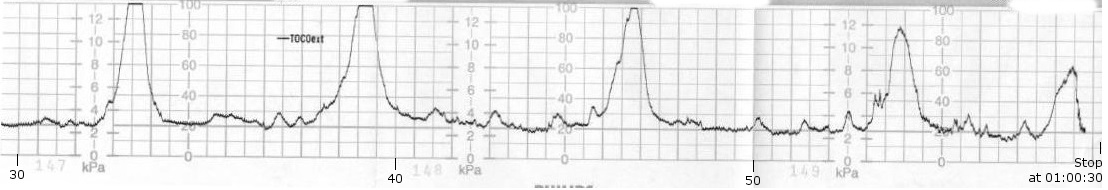
\includegraphics[scale=0.45]{imagens/toco.jpg} 		
 	\end{center}
 	%\legend{\cite{ref-islddatabase}}
 \end{figure}
 
 There are several disadvantages of Tocography. Important
 among them are:
 
 \begin{itemize}[leftmargin=*,labelsep=5.8mm]
 	\item	Inter and intra-personal variation in interpretation of CTG
 	trace \cite{ref-bernardes}.
 	\item	Sometimes there is shift (either up or down) in baseline of
 	signal which makes interpretation difficult. This is known as
 	baseline wandering \cite{ref-marques}. 	
 \end{itemize}
 
 The purpose of this work is to evaluate the possibility of early detection of preterm delivery (PD), by means
 of characterization of the contractions, obtained by uterine
 electromyogram (EMG), on the abdomen of the pregnant
 woman [electrohysterogram (EHG)], using fuzzy logic. As there is no current
 published information concerning fuzzy classification of EHG recordings, we propose to investigate, in this study, the potentialities of this method to determine a possible separation between contractions leading to a PD and contractions leading to
 delivery at term (DT), using fuzzy classification and avoiding CTG disavantages.



%Please use the command \citep{ref-journal} for the following MDPI journals, which use author-date citation: Arts, Econometrics, Economies, Genealogy, Humanities, IJFS, JRFM, Laws, Religions, Risks, Social Sciences.


%%%%%%%%%%%%%%%%%%%%%%%%%%%%%%%%%%%%%%%%%%
\section{Materials}

\subsection{The Icelandic 16-electrode	Electrohysterogram Database}


The acquisitions of this database were executed between 2008 and 2010 in the Landspitali University Hospital, Akureyri Hospital and Akureyri Primary Health Care Centre in Iceland. Were performed 122 recordings on 45 pregnant woman, where 32 were measured repeatedly during
the same pregnancy and participated in two to seven recordings. Sessions ocurred in the third
trimester (112 recordings) and during labor (10 recordings). The database includes simultaneously recorded tocographs, annotations of events and obstetric information on participants. Informed consent was obtained from every participant and the protocol was approved by the National
Bioethics Committee in Iceland (VSN 02-006-V4) \cite{ref-islddatabase}.


A $4x4$ reusable monopolar eletrode grid (Ag/AgCl) was disposed on the pacients abdomen as can be seen in Figure \ref{abd_elec} 


 \begin{figure}[H]
 	\caption{\label{abd_elec} Ideal position of the 16 electrode grid. The black dots represents the patient ground reference.}
 	\begin{center}
 		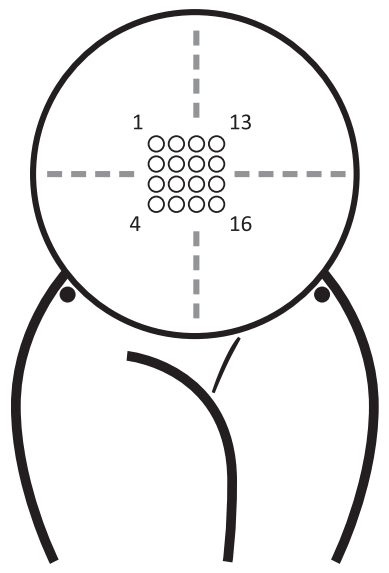
\includegraphics[scale=0.35]{imagens/abd_elec.png} 		
 	\end{center}
 	%\legend{\cite{ref-islddatabase}}
 \end{figure}

The measurements were performed using a sixteen channel multi-purpose physiological signal
recorder (Embla A10), most commonly used for investigating sleep disorders. An anti-aliasing filter with
a high cut-off frequency of 100 Hz was used but no high pass filter was used. The signal sampling rate was 200 Hz and the signal was digitized to 16 bits.  \cite{ref-islddatabase}.

\subsection{The Term-Preterm Electrohysterogram database}

The EHG records included in the Term-Preterm Electrohysterogram database (TPEHG DB) were obtained from 1997 to 2005 at the University Medical Centre Ljubljana, Department of Obstetrics and Gynecology. The records were obtained during regular check-ups either around the 22nd week of gestation or around the 32nd week of gestation. In all, almost 1300 records were obtained during these years, and a preliminary database was built and used for studies by Ivan Verdenik, Gorazd Kavšek, Marjan Pajntar and Živa Novak-Antolič \cite{ref-verdenik},\cite{ref-kavsek}

During the selection of records, all records with apparent recording artifacts, all records from pregnancies where labor was induced, and all records where delivery was performed using a Cesarean section, were rejected. The 300 resulted data are:

\begin{itemize}[leftmargin=*,labelsep=5.8mm]
	
	\item	262 records were obtained during pregnancies where delivery was on term (duration of gestation at delivery $>$ 37 weeks):
	
	\begin{itemize}[leftmargin=*,labelsep=5.8mm]
		\item 143 records were obtained before the 26th week of gestation and	
		
		\item 119 were obtained later during pregnancy, during or after the 26th week of gestation;	
	\end{itemize}
	
	\item	38 records were obtained during pregnancies which ended prematurely (pregnancy duration $\leq$ 37 weeks), of which:
	
	\begin{itemize}[leftmargin=*,labelsep=5.8mm]
		\item 19 records were obtained before the 26th week of gestation and
			
		\item	19 records were obtained during or after the 26th week of gestation.	
	\end{itemize}
	 	
\end{itemize}

The differences in the electrical potentials of the electrodes were recorded, producing 3 channels:

\begin{itemize}[leftmargin=*,labelsep=5.8mm]
	\item S1 = E2–E1 (first channel);
	\item S2 = E2–E3 (second channel);
	\item S3 = E4–E3 (third channel).
\end{itemize}

A $2x2$ reusable monopolar eletrode grid (Ag/AgCl) was disposed on the pacients abdomen as can be seen in Figure \ref{abd_elec4x4}. 

 \begin{figure}[H]
 	\caption{\label{abd_elec4x4} Ideal position of the 4 electrode grid. }
 	\begin{center}
 		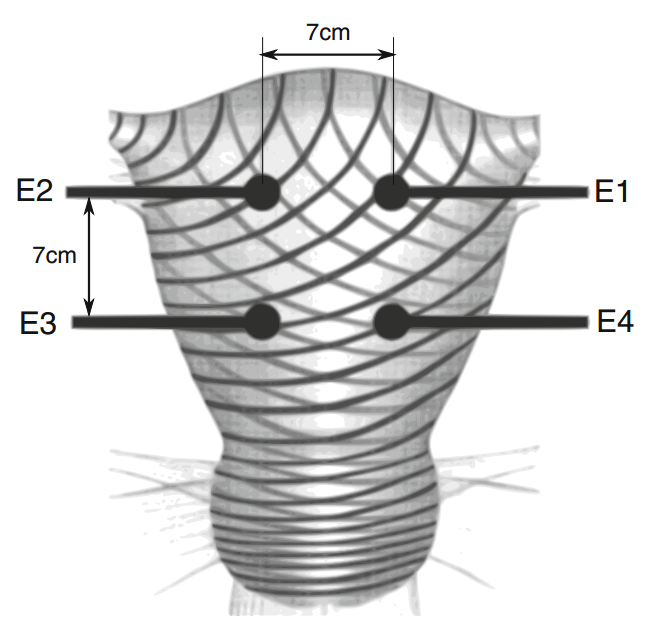
\includegraphics[scale=0.43]{imagens/abd_elec4x4.png} 		
 	\end{center}
 	%\legend{\cite{ref-islddatabase}}
 \end{figure}
 
 The records are of 30-min
 duration and consist of three channels. The sampling frequency was 20Hz and the signal was digitized to 16 bits. Prior to
 sampling the signals were filtered using an analog threepole Butterworth filter with the bandwidth from 0 to 5 Hz \cite{ref-baseboa}
 
 \subsection{The Fuzzy Logic}
 
 Unlike in the boolean logic, in the fuzzy logic the variables can assume more than 2 values (true and false). That is, it can work in the concept where the truth can range between the completely true to completely false \cite{ref-novak}
 
 
 
 %%%%%%%%%%%%%%%%%%%%%%%%%%%%%%%%%%%%%%%%%%
 \section{Methods}

 %%%%%%%%%%%%%%%%%%%%%%%%%%%%%%%%%%%%%%%%%%
 \subsection{Pre-Processing}
 
 The TPEHG database was chosen for providing more consistent data, information on the type of contraction (preterm and term) and using differential signals. Moreover, because it has been elaborated longer, it has more work based on its measurements, thus allowing the results obtained here to be compared in the future.
 
 The selection of digital filters to remove noise from signals
 before the processing may greatly influence the results.
 A band-pass filter is needed. It was recognized that the uterine
 EMG content ranges from 0 to $<$ 5 Hz \cite{ref-devedeux}.
 
 
 
 
 
 
 
 
 
 
 
 
 
 
 
 
 
 
 
 
 
 
 


 
 
%%%%%%%%%%%%%%%%%%%%%%%%%%%%%%%%%%%%%%%%%%
\section{Results}

This section may be divided by subheadings. It should provide a concise and precise description of the experimental results, their interpretation as well as the experimental conclusions that can be drawn.


%%%%%%%%%%%%%%%%%%%%%%%%%%%%%%%%%%%%%%%%%%
\subsection{Subsection}

\subsubsection{Subsubsection}

Bulleted lists look like this:
\begin{itemize}[leftmargin=*,labelsep=5.8mm]
\item	First bullet
\item	Second bullet
\item	Third bullet
\end{itemize}

Numbered lists can be added as follows:
\begin{enumerate}[leftmargin=*,labelsep=4.9mm]
\item	First item 
\item	Second item
\item	Third item
\end{enumerate}

The text continues here.

\subsection{Figures, Tables and Schemes}

All figures and tables should be cited in the main text as Figure 1, Table 1, etc.

 \begin{figure}[H]
 	\caption{\label{beer}This is a figure, Schemes follow the same formatting. If there are multiple panels, they should be listed as: (\textbf{a}) Description of what is contained in the first panel. (\textbf{b}) Description of what is contained in the second panel. Figures should be placed in the main text near to the first time they are cited. A caption on a single line should be centered.}
 	\begin{center}
 		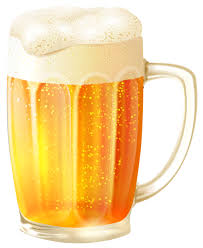
\includegraphics[scale=0.40]{imagens/beer.jpg} 		
 	\end{center}
 	%\legend{\cite[]{pll analog}}
 \end{figure}  



\begin{table}[H]
\caption{This is a table caption. Tables should be placed in the main text near to the first time they are cited.}
\centering
%% \tablesize{} %% You can specify the fontsize here, e.g.  \tablesize{\footnotesize}. If commented out \small will be used.
\begin{tabular}{ccc}
\toprule
\textbf{Title 1}	& \textbf{Title 2}	& \textbf{Title 3}\\
\midrule
entry 1		& data			& data\\
entry 2		& data			& data\\
\bottomrule
\end{tabular}
\end{table}

\subsection{Formatting of Mathematical Components}

This is an example of an equation:

\begin{equation}
\mathbb{S}
\end{equation}

%% If the documentclass option "submit" is chosen, please insert a blank line before and after any math environment (equation and eqnarray environments). This ensures correct linenumbering. The blank line should be removed when the documentclass option is changed to "accept" because the text following an equation should not be a new paragraph. 
Please punctuate equations as regular text. Theorem-type environments (including propositions, lemmas, corollaries etc.) can be formatted as follows:
%% Example of a theorem:
\begin{Theorem}
Example text of a theorem.
\end{Theorem}

The text continues here. Proofs must be formatted as follows:

%% Example of a proof:
\begin{proof}[Proof of Theorem 1]
Text of the proof. Note that the phrase `of Theorem 1' is optional if it is clear which theorem is being referred to.
\end{proof}
The text continues here.


%%%%%%%%%%%%%%%%%%%%%%%%%%%%%%%%%%%%%%%%%%
\section{Discussion}

Authors should discuss the results and how they can be interpreted in perspective of previous studies and of the working hypotheses. The findings and their implications should be discussed in the broadest context possible. Future research directions may also be highlighted.


%%%%%%%%%%%%%%%%%%%%%%%%%%%%%%%%%%%%%%%%%%
\section{Conclusions}

This section is not mandatory, but can be added to the manuscript if the discussion is unusually long or complex.

%%%%%%%%%%%%%%%%%%%%%%%%%%%%%%%%%%%%%%%%%%
\vspace{6pt} 





%%%%%%%%%%%%%%%%%%%%%%%%%%%%%%%%%%%%%%%%%%
\conflictsofinterest{The authors declare no conflict of interest.} 


%=====================================
% References, variant A: internal bibliography
%=====================================
\begin{thebibliography}{999}
	
%% Reference 1
\bibitem[T.L. Weissgerber, L.A. Wolfe (2006)]{ref-weisswolfe}
T.L. Weissgerber, L.A. Wolfe. Physiological adaptation in early human pregnancy: adaptation to balance maternal-fetal demands. {\em Appl. Physiol. Nutr. Metab.} {\bf 2006}, {\em 31}, 1-11.

%% Reference 2
\bibitem[Alkema L. {\em et al} (2016)]{ref-alkema}
Alkema L. {\em et al}. Global, regional, and national levels and trends in maternal mortality between 1990 and 2015, with scenario-based projections to 2030: a systematic analysis by the UN Maternal Mortality Estimation Inter-Agency Group. {\em Lancet} {\bf 2016}, {\em 387}, 462–74.

%% Reference 3
\bibitem[Villanueva L. A., Contreras A. K., Pichardo M., Rosales L. J. (2008)]{ref-villa}
Villanueva L. A., Contreras A. K., Pichardo M., Rosales L. J. Perfil epidemiológico del parto prematuro {\em Ginecol Obstet Mex.} {\bf 2008}, {\em 76}, 542-548. 

%% Reference 4
\bibitem[J. Bernardes, A. Costa-Pereira, D. Ayres-de-Campos, H. Van Geijn, and L. Pereira-Leite. (1997)]{ref-bernardes}
J. Bernardes, A. Costa-Pereira, D. Ayres-de-Campos, H. Van Geijn, and L. Pereira-Leite. Evaluation of interobserver agreement of Cardiotocograms {\em International Journal of Gynaecology \& Obstetrics.} {\bf 1997}, {\em 57}, 33-37.

%% Reference 5
\bibitem[J. A. Marques, P. C. Cortez, J. P. Madeiro, and F. S. Schlindwein (2013)]{ref-marques}
J. A. Marques, P. C. Cortez, J. P. Madeiro, and F. S. Schlindwein. Computerized Cardiotocography analysis system based on Hilbert Transform {\em Expert System with Applications.} {\bf 2013}, {\em 40}, 7159-7658.		
	
%% Reference 6
\bibitem[Alexandersson, A. { \em et al} (2015)]{ref-islddatabase}
Alexandersson, A. { \em et al}.  The Icelandic 16-electrode electrohysterogram database. {\em Sci. Data 2:150017} {\bf 2015}, doi: 10.1038/sdata.2015.17.

%% Reference 7
\bibitem[Verdenik, I. (2002)]{ref-verdenik}
Verdenik, I.  Multilayer prediction model for preterm delivery. {\em PhD thesis}, University of Ljubljana, Medical faculty, Ljubljana, 2002.

%% Reference 8
\bibitem[Kavšek, G. (2001)]{ref-kavsek}
Kavšek, G.  Electromyographic activity of the uterus in threatened preterm delivery. {\em MsC thesis}, University of Ljubljana, Medical faculty, Ljubljana, 2001.


%% Reference 9
\bibitem[Fele-Zorz G., Kavšek, G, Novak-Antolic Z., Jager F. (2008)]{ref-baseboa}
Fele-Zorz G., Kavšek, G, Novak-Antolic Z., Jager F.  A comparison of various linear and non-linear signal processing techniques to separate uterine EMG records of term and pre-term delivery groups. {\em Med Biol Eng Comput} {\bf 2008}, {\em 46}, 911–922.	

%% Reference 10
\bibitem[  Novák, V., Perfilieva, I., Močkoř, J. (1999)]{ref-novak}
Novák, V., Perfilieva, I., Močkoř, J. {\em Mathematical Principles of Fuzzy Logic}; 1st ed; Kluwer Academic Publishers: Boston,
USA, 1999; ISBN 0-7923-8595-0

%% Reference 11
\bibitem[Devedeux D., Marque C., Mansour S., Germain G., Duchene J. (1993)]{ref-devedeux}
Devedeux D., Marque C., Mansour S., Germain G., Duchene J. Uterine electromyography: a critical review. {\em Am J Obstet Gynecol} {\bf 1993}, {\em 169(6)}, 1636–1653.	





	
 



%% Reference expl
%\bibitem[Author (year)]{ref-journal}
%Lastname, F.; Author, T. The title of the cited article. {\em Journal Abbreviation} {\bf 2008}, {\em %10}, 142-149.

%% Reference 2
%\bibitem[Author (year)]{ref-book}
%Lastname, F.F.; Author, T. The title of the cited contribution. In {\em The Book Title}; Editor, F., Meditor, A., Eds.; Publishing House: City, Country, 2007; pp. 32-58.
\end{thebibliography}

% The following MDPI journals use author-date citation: Arts, Econometrics, Economies, Genealogy, Humanities, IJFS, JRFM, Laws, Religions, Risks, Social Sciences. For those journals, please follow the formatting guidelines on http://www.mdpi.com/authors/references

%=====================================
% References, variant B: external bibliography
%=====================================
%\externalbibliography{yes}
%\bibliography{references}

%%%%%%%%%%%%%%%%%%%%%%%%%%%%%%%%%%%%%%%%%%
%% optional
%\sampleavailability{Samples of the compounds ...... are available from the authors.}

%%%%%%%%%%%%%%%%%%%%%%%%%%%%%%%%%%%%%%%%%%
\end{document}

